%
% rhs.tex
%
% (c) 2018 Prof Dr Andreas Müller, Hochschule Rapperswil
%
\documentclass[tikz]{standalone}
\usepackage{times}
\usepackage{amsmath}
\usepackage{txfonts}
\usepackage[utf8]{inputenc}
\usepackage{graphics}
\usetikzlibrary{arrows,intersections}
\begin{document}
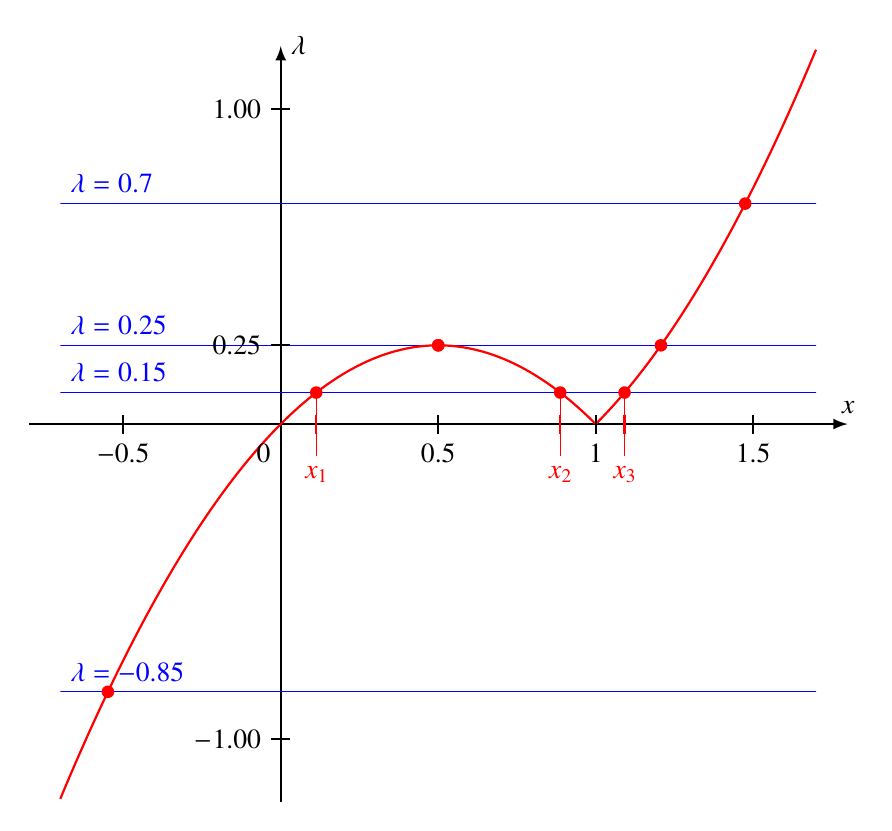
\begin{tikzpicture}[thick, >= latex, scale=4]

\draw[->] (-0.8,0)--(1.8,0) coordinate[label={above:$x$}];
\draw[->] (0,-1.2)--(0,1.2) coordinate[label={right:$\lambda$}];

\begin{scope}
\clip (-0.7,-1.2) rectangle (1.7,1.2);
\draw[line width=0.5,color=blue] (-2,0.7)--(2,0.7);
\node[color=blue] at (-0.7,0.7) [above right] {$\lambda=0.7$};
\draw[line width=0.5,color=blue] (-2,0.25)--(2,0.25);
\node[color=blue] at (-0.7,0.25) [above right] {$\lambda=0.25$};
\draw[line width=0.5,color=blue] (-2,0.1)--(2,0.1);
\node[color=blue] at (-0.7,0.1) [above right] {$\lambda=0.15$};
\draw[line width=0.5,color=blue] (-2,-0.85)--(2,-0.85);
\node[color=blue] at (-0.7,-0.85) [above right] {$\lambda=-0.85$};
\end{scope}

\draw[domain=1:1.7,samples=100,color=red] plot ({\x},{(\x-1)*\x});
\draw[domain=-0.7:1,samples=100,color=red] plot({\x},{(1-\x)*\x});

\fill[color=red] (0.5,0.25) circle[radius=0.02];
\fill[color=red] (0.5,0.25) circle[radius=0.02];

\fill[color=red] ({0.5-sqrt(0.25-0.1)},{0.1}) circle[radius=0.02];
\fill[color=red] ({0.5+sqrt(0.25-0.1)},{0.1}) circle[radius=0.02];
\fill[color=red] ({0.5+sqrt(0.25+0.1)},{0.1}) circle[radius=0.02];

\fill[color=red] ({0.5+sqrt(0.25+0.25)},{0.25}) circle[radius=0.02];

\fill[color=red] ({0.5+sqrt(0.25+0.7)},{0.7}) circle[radius=0.02];

\fill[color=red] ({0.5-sqrt(0.25+0.85)},{-0.85}) circle[radius=0.02];

\draw    ( 1.0,-0.03)--( 1.0,0.03);
\node at ( 1.0,-0.03) [below] {$1$};
\draw    ( 0.5,-0.03)--( 0.5,0.03);
\draw    ( 1.5,-0.03)--( 1.5,0.03);
\draw    (-0.5,-0.03)--(-0.5,0.03);
\node at ( 0.5,-0.03) [below] {$0.5$};
\node at (-0.5,-0.03) [below] {$-0.5$};
\node at ( 1.5,-0.03) [below] {$1.5$};
\node at ( 0.0,-0.03) [below left] {$0$};


\draw    (-0.03, 0.25)--(0.03,0.25);
\node at (-0.03, 0.25) [left] {$0.25$};
\draw    (-0.03, 1.00)--(0.03,1);
\draw    (-0.03,-1.00)--(0.03,-1);
\node at (-0.03, 1.00) [left] {$1.00$};
\node at (-0.03,-1.00) [left] {$-1.00$};

\draw[color=red,line width=0.5] ({0.5-sqrt(0.25-0.1)},0.1)
	--({0.5-sqrt(0.25-0.1)},-0.1);
\draw[color=red] ({0.5-sqrt(0.25-0.1)},0.03)--({0.5-sqrt(0.25-0.1)},-0.03);
\node[color=red] at ({0.5-sqrt(0.25-0.1)},-0.1) [below] {$x_1$};

\draw[color=red,line width=0.5] ({0.5+sqrt(0.25-0.1)},0.1)
	--({0.5+sqrt(0.25-0.1)},-0.1);
\draw[color=red] ({0.5+sqrt(0.25-0.1)},0.03)--({0.5+sqrt(0.25-0.1)},-0.03);
\node[color=red] at ({0.5+sqrt(0.25-0.1)},-0.1) [below] {$x_2$};

\draw[color=red,line width=0.5] ({0.5+sqrt(0.25+0.1)},0.1)
	--({0.5+sqrt(0.25+0.1)},-0.1);
\draw[color=red] ({0.5+sqrt(0.25+0.1)},0.03)--({0.5+sqrt(0.25+0.1)},-0.03);
\node[color=red] at ({0.5+sqrt(0.25+0.1)},-0.1) [below] {$x_3$};

\end{tikzpicture}
\end{document}

